\documentclass[aspectratio=169]{beamer}

\usetheme{Madrid}
\usecolortheme{default}

\usepackage[utf8]{inputenc}
\usepackage[T1]{fontenc}
\usepackage{amsmath}
\usepackage{amssymb}
\usepackage{booktabs}
\usepackage{array}
\usepackage{listings}
\usepackage{xcolor}
\usepackage{colortbl}
\usepackage{graphicx}
\usepackage{hyperref}

\hypersetup{
    colorlinks=true,
    linkcolor=blue,
    citecolor=blue,
    urlcolor=blue
}

% =========================================================
% COLORS
% =========================================================
\definecolor{navy}{RGB}{23,55,105}
\definecolor{blueaccent}{RGB}{40,105,180}
\definecolor{lightblue}{RGB}{233,242,252}
\definecolor{lightgray}{RGB}{246,248,251}
\definecolor{midgray}{RGB}{105,115,130}
\definecolor{darktext}{RGB}{35,43,56}
\definecolor{success}{RGB}{21,122,72}
\definecolor{errorred}{RGB}{176,0,32}
\definecolor{codegreen}{RGB}{0,110,85}

% =========================================================
% GLOBAL APPEARANCE
% =========================================================
\setbeamercolor{normal text}{fg=darktext,bg=white}
\setbeamercolor{structure}{fg=navy}
\setbeamercolor{alerted text}{fg=errorred}

\setbeamerfont{title}{series=\bfseries,size=\LARGE}
\setbeamerfont{subtitle}{size=\large}
\setbeamerfont{frametitle}{series=\bfseries,size=\large}
\setbeamerfont{block title}{series=\bfseries}
\setbeamerfont{footline}{size=\scriptsize}

\setbeamertemplate{navigation symbols}{}
\setbeamertemplate{itemize items}[circle]
\setbeamertemplate{itemize subitem}[dash]

\setlength{\parskip}{0.35em}
\setlength{\tabcolsep}{7pt}
\renewcommand{\arraystretch}{1.22}

% =========================================================
% FRAME TITLE
% =========================================================
\setbeamercolor{frametitle}{fg=white,bg=navy}

\setbeamertemplate{frametitle}{
    \nointerlineskip
    \begin{beamercolorbox}[
        wd=\paperwidth,
        ht=2.9ex,
        dp=1.15ex,
        leftskip=0.45cm
    ]{frametitle}
        \insertframetitle
    \end{beamercolorbox}
    \vspace{0.18cm}
}

% =========================================================
% BLOCKS / CARDS
% =========================================================
\setbeamercolor{block title}{fg=white,bg=navy}
\setbeamercolor{block body}{fg=darktext,bg=lightblue}

\setbeamercolor{block title alerted}{fg=white,bg=errorred}
\setbeamercolor{block body alerted}{fg=darktext,bg=red!7}

\setbeamercolor{block title example}{fg=white,bg=success}
\setbeamercolor{block body example}{fg=darktext,bg=green!7}

\setbeamertemplate{blocks}[rounded][shadow=false]

% =========================================================
% TABLE
% =========================================================
\newcommand{\tableheader}[1]{%
    \multicolumn{1}{c}{\color{white}\textbf{#1}}%
}

% =========================================================
% FOOTER
% =========================================================
\setbeamercolor{author in head/foot}{fg=white,bg=navy}
\setbeamercolor{title in head/foot}{fg=white,bg=navy}
\setbeamercolor{date in head/foot}{fg=white,bg=navy}

\setbeamertemplate{footline}{
    \leavevmode%
    \hbox{%
        \begin{beamercolorbox}[
            wd=.34\paperwidth,
            ht=2.7ex,
            dp=1.15ex,
            left,
            leftskip=0.32cm
        ]{author in head/foot}
            \usebeamerfont{footline}
            Mohammad Aliyawar Khan
        \end{beamercolorbox}%

        \begin{beamercolorbox}[
            wd=.42\paperwidth,
            ht=2.7ex,
            dp=1.15ex,
            center
        ]{title in head/foot}
            \usebeamerfont{footline}
            \textbf{SOEN 6011 -- Deliverable 2}
        \end{beamercolorbox}%

        \begin{beamercolorbox}[
            wd=.24\paperwidth,
            ht=2.7ex,
            dp=1.15ex,
            right,
            rightskip=0.32cm
        ]{date in head/foot}
            \usebeamerfont{footline}
            \insertframenumber/\inserttotalframenumber
        \end{beamercolorbox}%
    }%
}

% =========================================================
% PYTHON LISTING STYLE
% =========================================================
\lstdefinestyle{pythonstyle}{
    language=Python,
    basicstyle=\ttfamily\scriptsize\color{darktext},
    keywordstyle=\color{blueaccent}\bfseries,
    commentstyle=\color{midgray}\itshape,
    stringstyle=\color{codegreen},
    showstringspaces=false,
    numbers=none,
    frame=single,
    rulecolor=\color{navy!35},
    backgroundcolor=\color{lightgray},
    breaklines=true,
    breakatwhitespace=true,
    tabsize=4,
    xleftmargin=1.2em,
    framexleftmargin=1em,
    aboveskip=0.25cm,
    belowskip=0.15cm
}

% =========================================================
% METADATA
% =========================================================
\title{SOEN 6011 -- Deliverable 2}
\subtitle{F1: \(\arccos(x)\) Calculator}
\author{Mohammad Aliyawar Khan}
\institute{Concordia University}
\date{Summer 2026}

\begin{document}

% =========================================================
% TITLE
% =========================================================
\begin{frame}[plain]
\centering
\vspace{0.65cm}

{\color{navy}\rule{0.82\textwidth}{1.4pt}\par}
\vspace{0.55cm}

{\usebeamerfont{title}\color{navy}SOEN 6011 - Deliverable 2\par}
\vspace{0.12cm}

{\color{blueaccent}\Large F1: \(\arccos(x)\) Calculator\par}
\vspace{0.7cm}


\vfill

{\large Mohammad Aliyawar Khan\par}
\vspace{0.10cm}
{\normalsize Student ID: 40309082 \quad | \quad Concordia University, Montreal\par}
\vspace{0.12cm}
{\normalsize Summer 2026\par}

\vspace{0.45cm}
{\color{navy}\rule{0.82\textwidth}{1.4pt}\par}
\end{frame}

% =========================================================
% SCOPE
% =========================================================
\begin{frame}{Deliverable 2 Scope}
\small

\begin{columns}[T,onlytextwidth]

\column{0.30\textwidth}
\begin{block}{Problem 5}
\centering
\textbf{Implementation}

\vspace{0.05cm}

\begin{itemize}
    \item Tkinter GUI
    \item From-scratch \(\arccos(x)\)
    \item Validation and recovery
\end{itemize}
\end{block}

\column{0.30\textwidth}
\begin{block}{Problem 6}
\centering
\textbf{Repository}

\vspace{0.05cm}

\begin{itemize}
    \item Public GitHub
    \item README
    \item Meaningful commits
\end{itemize}
\end{block}

\column{0.30\textwidth}
\begin{block}{Problem 7}
\centering
\textbf{Requirements}

\vspace{0.05cm}

\begin{itemize}
    \item Updated D2 requirements
    \item Testable statements
    \item Code evidence
\end{itemize}
\end{block}

\end{columns}

\vspace{0.08cm}

\begin{exampleblock}{Key D2 Outcome}
The D1 textual calculator became a Tkinter GUI with range reduction,
numerical verification, error recovery, and repository documentation.
\end{exampleblock}

\vspace{-0.05cm}

\begin{block}{Retained D1 Constraints}
Valid domain: \([-1,1]\) \quad
Principal range: \([0,\pi]\) \quad
Accuracy target: \(\leq 10^{-6}\) radians
\scriptsize\cite{project}
\end{block}


\end{frame}

% =========================================================
% REQUIREMENTS
% =========================================================
\begin{frame}{Key Updated Requirements}
\small
\rowcolors{2}{lightgray}{white}
\begin{tabular}{p{0.20\textwidth}p{0.67\textwidth}}
\rowcolor{navy}
\tableheader{ID} & \tableheader{Requirement Summary} \\
\toprule
FR-001--003 & Tkinter GUI, numeric input field, and Calculate control. \\
FR-004--005 & Reject non-finite values and values outside \([-1,1]\). \\
FR-006--008 & Compute \(\arccos(x)\) from scratch and display radians in \([0,\pi]\). \\
FR-009--013 & Helpful error messages, recovery, Clear, and Exit controls. \\
NFR-001 & Execute using Python 3.x in an environment that supports Tkinter. \\
NFR-002 & Tested valid results must have absolute error no greater than \(10^{-6}\) radians. \\
NFR-003--004 & Numerical iteration limits and modular separation of responsibilities. \\
\bottomrule
\end{tabular}

\vspace{0.28cm}

\begin{block}{Requirements Evidence}
Complete requirements and traceability are presented in the following slides.
\small\cite{project,iso29148}
\end{block}

\end{frame}

% =========================================================
% SECTION 
% =========================================================
\begin{frame}[plain]
\centering
\vfill
{\color{navy}\LARGE\bfseries Application Experience\par}
\vspace{0.2cm}
{\large GUI workflow, validation, and error recovery\par}
\vfill
\end{frame}

% =========================================================
% GUI
% =========================================================
\begin{frame}{Tkinter Interface and User Flow}
\centering

\begin{minipage}{0.43\textwidth}
\centering
\fcolorbox{navy!35}{lightgray}{
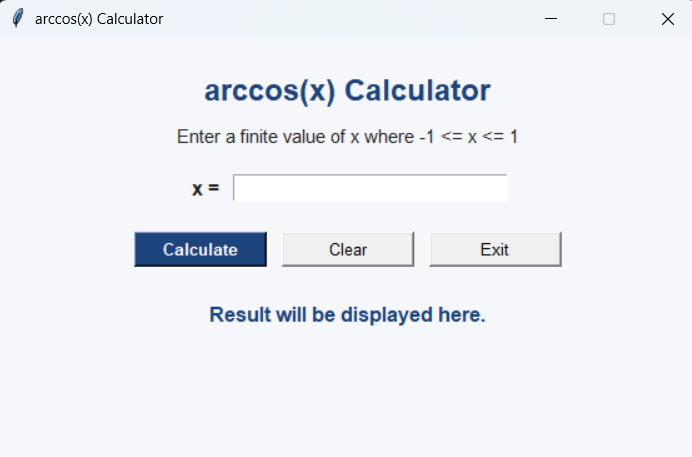
\includegraphics[
    width=0.95\textwidth,
    height=0.46\textheight,
    keepaspectratio
]{tkinter_b.png}
}

\vspace{0.10cm}
\small\color{midgray}Input interface
\end{minipage}
\hfill
\begin{minipage}{0.43\textwidth}
\centering
\fcolorbox{navy!35}{lightgray}{
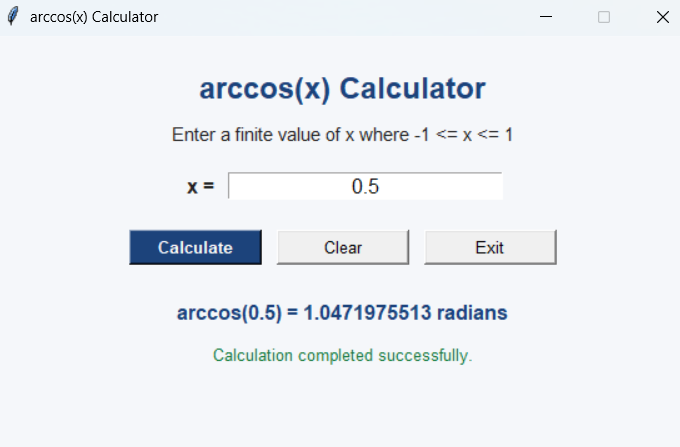
\includegraphics[
    width=0.95\textwidth,
    height=0.46\textheight,
    keepaspectratio
]{tkinter_a.png}
}

\vspace{0.10cm}
\small\color{midgray}Successful calculation
\end{minipage}

\vspace{0.25cm}

\begin{exampleblock}{User Flow}
Enter \(x\), select \textbf{Calculate} or press Enter, receive a result or
helpful error message, then correct input and calculate again without restarting.
\end{exampleblock}
\end{frame}

% =========================================================
% VALIDATION
% =========================================================
\begin{frame}{Input Validation and Error Recovery}
\small
\rowcolors{2}{lightgray}{white}
\begin{tabular}{p{0.31\textwidth}p{0.55\textwidth}}
\rowcolor{navy}
\tableheader{Condition} & \tableheader{Application Behaviour} \\
\toprule
Empty input & Requests a finite input in the interval \([-1,1]\). \\
Text such as \texttt{hello} & Requests numeric input such as \(0\), \(0.5\), or \(-0.75\). \\
\texttt{nan}, \texttt{inf}, or \texttt{-inf} & Rejects the value as non-finite. \\
\(x < -1\) or \(x > 1\) & Explains the valid domain \([-1,1]\). \\
Iteration limit reached & Displays a convergence-error message. \\
\bottomrule
\end{tabular}

\vspace{0.35cm}

\begin{columns}[T,onlytextwidth]
\column{0.48\textwidth}
\begin{alertblock}{Custom Exceptions}
\texttt{InputValidationError}\\
\texttt{ConvergenceError}
\end{alertblock}

\column{0.48\textwidth}
\begin{exampleblock}{Recovery}
The GUI catches errors and immediately allows another calculation.
\end{exampleblock}
\end{columns}
\end{frame}

% =========================================================
% SECTION 
% =========================================================
\begin{frame}[plain]
\centering
\vfill
{\color{navy}\LARGE\bfseries Numerical Design\par}
\vspace{0.2cm}
{\large Range reduction, Taylor recurrence, and Newton's method\par}
\vfill
\end{frame}

% =========================================================
% METHOD
% =========================================================
\begin{frame}{Taylor Series with Range Reduction}
\begin{columns}[T,onlytextwidth]
\column{0.50\textwidth}

\begin{alertblock}{Why reduction is needed}
Direct Taylor-series evaluation of \(\arcsin(x)\) converges slowly when
\(\lvert x\rvert\) is close to \(1\).
\end{alertblock}

\begin{block}{For nonnegative input}
\[
\arccos(x)=
2\arcsin\left(\sqrt{\frac{1-x}{2}}\right)
\]

The transformed input becomes small when \(x\) is close to \(1\).
\end{block}

\column{0.46\textwidth}

\begin{block}{For negative input}
\[
\arccos(x)=\pi-\arccos(-x)
\]

The negative branch is converted to a nonnegative calculation.
\end{block}

\begin{exampleblock}{From-scratch components}
\begin{itemize}
    \item \(\arcsin(x)\): Taylor recurrence
    \item \(\sqrt{x}\): Newton's method
    \item Endpoints: direct returns
\end{itemize}
\end{exampleblock}
\end{columns}

\small\cite{stewart,burden}
\end{frame}

% =========================================================
% ARCCOS CODE
% =========================================================
\begin{frame}[fragile]{Final Code: Range-Reduced \texttt{arccos}}

\begin{lstlisting}[
    style=pythonstyle,
    basicstyle=\ttfamily\tiny\color{darktext},
    aboveskip=0.12cm,
    belowskip=0cm
]
def calculate_arccos(x):
    if not is_finite_number(x):
        raise InputValidationError(
            "Enter a finite number. Values such as nan are not allowed."
        )

    if x < -1.0 or x > 1.0:
        raise InputValidationError(
            "Input is outside the valid domain. Enter a value from -1 to 1."
        )

    if x == 1.0:
        return 0.0
    if x == -1.0:
        return PI
    if x < 0.0:
        return PI - calculate_arccos(-x)

    reduced_input = calculate_square_root((1.0 - x) / 2.0)
    return 2.0 * calculate_arcsin(reduced_input)
\end{lstlisting}

\vspace{-0.10cm}
\scriptsize\textit{Exact excerpt from the final \texttt{problem5.py} implementation.}

\end{frame}

% =========================================================
% ARCSIN CODE
% =========================================================
\begin{frame}[fragile]{Taylor-Series Recurrence}

\begin{lstlisting}[
    style=pythonstyle,
    basicstyle=\ttfamily\tiny\color{darktext},
    aboveskip=0.10cm,
    belowskip=0cm
]
def calculate_arcsin(x):
    if x == 0.0:
        return 0.0

    result = 0.0
    coefficient = 1.0
    power = x
    iteration = 0

    while iteration < MAX_ITERATIONS:
        term = coefficient * power
        result = result + term

        if absolute_value(term) <= TOLERANCE:
            return result

        iteration = iteration + 1
        coefficient = (
            coefficient
            * (2 * iteration - 1)
            * (2 * iteration - 1)
            / ((2 * iteration) * (2 * iteration + 1))
        )
        power = power * x * x

    raise ConvergenceError(
        "Taylor-series calculation did not converge."
    )
\end{lstlisting}
\end{frame}

% =========================================================
% SQRT CODE
% =========================================================
\begin{frame}[fragile]{Newton Square-Root Calculation}

\begin{lstlisting}[
    style=pythonstyle,
    basicstyle=\ttfamily\tiny\color{darktext},
    aboveskip=0.10cm,
    belowskip=0cm
]
def calculate_square_root(value):
    if value < 0.0:
        raise InputValidationError(
            "Square root input must be greater than or equal to zero."
        )

    if value == 0.0:
        return 0.0

    guess = 1.0
    iteration = 0

    while iteration < SQRT_MAX_ITERATIONS:
        next_guess = 0.5 * (guess + value / guess)

        if absolute_value(next_guess - guess) <= SQRT_TOLERANCE:
            return next_guess

        guess = next_guess
        iteration = iteration + 1

    raise ConvergenceError(
        "Square-root calculation did not converge."
    )
\end{lstlisting}

\vspace{-0.12cm}
\scriptsize
Newton's method calculates \(\sqrt{(1-x)/2}\) without using \texttt{math.sqrt()}.
\end{frame}

% =========================================================
% SECTION
% =========================================================
\begin{frame}[plain]
\centering
\vfill
{\color{navy}\LARGE\bfseries Verification and Evidence\par}
\vspace{0.2cm}
{\large Accuracy results, repository, requirements, and demonstration\par}
\vfill
\end{frame}

% =========================================================
% VERIFICATION
% =========================================================
\begin{frame}{Numerical Verification Results}
\centering

\begin{exampleblock}{Accuracy Requirement Met}
All tested valid inputs satisfy:
\[
\left|\text{program result}-\text{reference value}\right|
\leq 10^{-6}\text{ radians}
\]
\end{exampleblock}

\vspace{0.10cm}

\scriptsize
\rowcolors{2}{lightgray}{white}
\begin{tabular}{c c c c}
\rowcolor{navy}
\tableheader{Input \(x\)} &
\tableheader{Program result} &
\tableheader{Reference value} &
\tableheader{Absolute error} \\
\toprule
\(-1.0000\) & 3.141592653590 & 3.141592653590 & 0.00e+00 \\
\(-0.9999\) & 3.127450400112 & 3.127450400112 & 0.00e+00 \\
\(0.0000\) & 1.570796326619 & 1.570796326795 & 1.76e-10 \\
\(0.5000\) & 1.047197551172 & 1.047197551197 & 2.48e-11 \\
\(0.9990\) & 0.044725087169 & 0.044725087169 & 8.33e-17 \\
\(0.9999\) & 0.014142253478 & 0.014142253478 & 7.81e-17 \\
\(1.0000\) & 0.000000000000 & 0.000000000000 & 0.00e+00 \\
\bottomrule
\end{tabular}

\vspace{0.18cm}

\scriptsize
Reference values were generated using Python \texttt{math.acos()} only for
verification; the application does not call this function.
\end{frame}

% =========================================================
% REPOSITORY
% =========================================================
\begin{frame}{Repository and Demonstration}
\begin{block}{Public GitHub Repository}
\centering
\href{https://github.com/md-aliyawar-khan/SOEN-6011-D2-arccos-calculator}
{\color{blueaccent}\texttt{github.com/md-aliyawar-khan/SOEN-6011-D2-arccos-calculator}}
\end{block}

\vspace{0.20cm}

\begin{columns}[T,onlytextwidth]
\column{0.48\textwidth}

\begin{block}{Contents at Submission}
\begin{itemize}
    \item \texttt{README.md}
    \item \texttt{problem5.py}
    \item  \texttt{Documentation}
\end{itemize}
\end{block}

\column{0.48\textwidth}

\begin{exampleblock}{Live Demonstration}
\begin{itemize}
    \item Valid and endpoint input
    \item Invalid-input recovery
    \item Another calculation without restart
    \item Clear and Exit controls
\end{itemize}
\end{exampleblock}
\end{columns}

\vfill
\centering
{\color{midgray}\small Documentation, source code, and meaningful commits are publicly available through the GitHub repository.}
\end{frame}

% =========================================================
% DEMO CHECKLIST
% =========================================================
\begin{frame}{Demonstration Checklist}
\small
\rowcolors{2}{lightgray}{white}
\begin{tabular}{p{0.25\textwidth}p{0.22\textwidth}p{0.42\textwidth}}
\rowcolor{navy}
\tableheader{Case} & \tableheader{Input} & \tableheader{Expected Outcome} \\
\toprule
Normal calculation & \(0.5\) & Displays approximately \(1.0471975512\) radians. \\
Near upper endpoint & \(0.9999\) & Displays approximately \(0.0141422535\) radians. \\
Lower endpoint & \(-1\) & Displays \(\pi\) radians. \\
Outside domain & \(2\) & Displays a domain-validation error. \\
Non-finite input & \texttt{nan} & Displays a finite-number error. \\
Invalid text & \texttt{hello} & Displays a numeric-input error. \\
Recovery & Error, then \(0\) & Accepts new input without restarting. \\
Exit & Exit button & Closes the application. \\
\bottomrule
\end{tabular}
\end{frame}

% =========================================================
% TRACEABILITY
% =========================================================
\begin{frame}{Selected Requirement-to-Code Traceability}
\scriptsize
\rowcolors{2}{lightgray}{white}
\begin{tabular}{p{0.20\textwidth}p{0.62\textwidth}}
\rowcolor{navy}
\tableheader{Requirement} & \tableheader{Final Implementation Evidence} \\
\toprule
FR-001--003 & \texttt{ArccosCalculatorGUI}, entry field, Calculate button, and Enter-key binding. \\
FR-004--005 & \texttt{is\_finite\_number(x)} and domain checks in \texttt{calculate\_arccos(x)}. \\
FR-006--008 & \texttt{calculate\_arccos()}, Taylor-series \texttt{calculate\_arcsin()}, and radians output label. \\
FR-009, FR-011 & GUI catches errors, displays feedback, and accepts another calculation. \\
FR-010 & Direct returns for \(x=1\) and \(x=-1\). \\
FR-012--013 & \texttt{clear\_fields()} and \texttt{self.window.destroy()}. \\
NFR-002 & Numerical-verification table with tested error below \(10^{-6}\). \\
NFR-003--004 & Iteration limits plus separate GUI, validation, and numerical functions. \\
\bottomrule
\end{tabular}

\vspace{0.20cm}

\begin{block}{Scope of This Table}
Selected examples are shown; the repository contains the complete final implementation.
\end{block}
\end{frame}

% =========================================================
% FUNCTIONAL REQUIREMENTS I
% =========================================================
\begin{frame}{Complete Functional Requirements I}
\scriptsize
\rowcolors{2}{lightgray}{white}
\begin{tabular}{p{0.14\textwidth}p{0.74\textwidth}}
\rowcolor{navy}
\tableheader{ID} & \tableheader{Requirement} \\
\toprule
FR-001 & The system shall provide a graphical user interface implemented using Tkinter. \\
FR-002 & The graphical user interface shall provide a text-entry field through which the user can enter one real-number value \(x\). \\
FR-003 & The system shall provide a Calculate button that initiates calculation of \(\arccos(x)\). \\
FR-004 & The system shall validate that the input is a finite numeric value. \\
FR-005 & The system shall validate that the input value is within the domain \([-1,1]\), inclusive. \\
FR-006 & For valid input, the system shall calculate \(\arccos(x)\) using a numerical implementation written from scratch in Python. \\
FR-007 & The system shall not use built-in or library functions for the mathematical computation of \(\arccos(x)\) or its subordinate numerical functions. \\
\bottomrule
\end{tabular}
\end{frame}

% =========================================================
% FUNCTIONAL REQUIREMENTS II
% =========================================================
\begin{frame}{Complete Functional Requirements II}
\scriptsize
\rowcolors{2}{lightgray}{white}
\begin{tabular}{p{0.14\textwidth}p{0.74\textwidth}}
\rowcolor{navy}
\tableheader{ID} & \tableheader{Requirement} \\
\toprule
FR-008 & The system shall display the calculated principal result in radians, where \(0 \leq \arccos(x) \leq \pi\). \\
FR-009 & If a nonnumeric, non-finite, or out-of-domain value is entered, the system shall display a helpful error message explaining the problem and valid input condition. \\
FR-010 & The system shall handle \(x=1\) and \(x=-1\) directly, returning \(0\) and \(\pi\), respectively. \\
FR-011 & The system shall allow the user to correct invalid input and perform another calculation without restarting the application. \\
FR-012 & The system shall provide a Clear control that removes current input and result or error feedback. \\
FR-013 & The system shall provide an Exit control that closes the application. \\
\bottomrule
\end{tabular}
\end{frame}

% =========================================================
% NON-FUNCTIONAL REQUIREMENTS
% =========================================================
\begin{frame}{Complete Non-Functional Requirements}
\scriptsize
\rowcolors{2}{lightgray}{white}
\begin{tabular}{p{0.14\textwidth}p{0.74\textwidth}}
\rowcolor{navy}
\tableheader{ID} & \tableheader{Requirement} \\
\toprule
NFR-001 & The application shall execute using Python 3.x in an environment that supports Tkinter, without requiring a particular IDE. \\
NFR-002 & For tested valid inputs, the absolute error compared with a trusted reference value shall not exceed \(10^{-6}\) radians. \\
NFR-003 & The Taylor-series and square-root calculations shall stop and display a convergence-related error message if configured iteration limits are reached. \\
NFR-004 & The source code shall separate GUI event handling, validation, numerical calculation, and result or error display into distinct functions. \\
NFR-005 & Error messages shall identify the cause of the problem and state the valid input condition where applicable. \\
NFR-006 & The GUI shall provide readable input, Calculate, Clear, Exit, result, and error-feedback areas. \\
\bottomrule
\end{tabular}
\end{frame}

% =========================================================
% GAI AND CASTROFF
% =========================================================
\begin{frame}[t]{GAI and CASTROFF: Problems 5--7}
\fontsize{7.7pt}{9.0pt}\selectfont
\setlength{\parskip}{0.12em}

\begin{block}{Problem 5 -- Implementation Review}
\textit{Prompt:} Review a from-scratch Taylor-series \(\arccos(x)\) Tkinter
implementation; identify endpoint-convergence risks, validation gaps, and
tests for a \(10^{-6}\)-radian target.

\textit{Decision:} Accepted range reduction; added custom exceptions and
iteration limits; rejected built-in inverse-trigonometric functions.
\end{block}

\vspace{0.05cm}

\begin{block}{Problem 6 -- Repository and README}
\textit{Prompt:} Draft a concise README for a Python Tkinter
\(\arccos(x)\) calculator: prerequisites, run command, method, testing,
and limitations.

\textit{Decision:} Accepted README structure; corrected the command to
\texttt{python problem5.py}; removed nonexistent-file references.
\end{block}

\vspace{0.05cm}

\begin{block}{Problem 7 -- Requirements Revision}
\textit{Prompt:} Review D2 requirements for clarity, testability, and
consistency with Tkinter and the from-scratch numerical method.

\textit{Decision:} Revised subjective statements into testable requirements
and linked them to final implementation evidence.
\end{block}

\vspace{0.06cm}

\centering
\color{midgray}
\textit{CASTROFF applied: context, task, constraints, expected output,
validation criteria, and review against final evidence.}
\end{frame}
% =========================================================
% CONCLUSION
% =========================================================
\begin{frame}{Conclusion}
\begin{columns}[T,onlytextwidth]
\column{0.48\textwidth}

\begin{block}{Delivered}
\begin{itemize}
    \item Tkinter GUI replacing the D1 text interface
    \item From-scratch numerical \(\arccos(x)\)
    \item Validation, recovery, Clear, and Exit controls
\end{itemize}
\end{block}

\column{0.48\textwidth}

\begin{exampleblock}{Verified}
\begin{itemize}
    \item Range reduction improves endpoint convergence
    \item All tested values met \(10^{-6}\)-radian accuracy
    \item Public repository includes source and README
\end{itemize}
\end{exampleblock}
\end{columns}

\vfill

\centering
{\color{navy}\Large\bfseries
F1: \(\arccos(x)\) delivered as a verified Tkinter application.\par}
\vspace{0.25cm}
{\color{blueaccent}\rule{0.72\textwidth}{1pt}\par}
\end{frame}

% =========================================================
% REFERENCES
% =========================================================
\begin{frame}[allowframebreaks]{References}
\footnotesize
\begin{thebibliography}{99}

\bibitem{project}
Concordia University, Department of Computer Science and Software Engineering,
\emph{SOEN 6011 Project Description},
Summer 2026.

\bibitem{iso29148}
ISO/IEC/IEEE,
\emph{ISO/IEC/IEEE 29148: Systems and Software Engineering --
Life Cycle Processes -- Requirements Engineering},
2018.

\bibitem{stewart}
James Stewart,
\emph{Calculus: Early Transcendentals},
Cengage Learning.

\bibitem{burden}
Richard L. Burden and J. Douglas Faires,
\emph{Numerical Analysis},
Cengage Learning.

\bibitem{python}
Python Software Foundation,
\emph{Python Documentation},
available at: \url{https://docs.python.org/3/}.

\bibitem{tkinter}
Python Software Foundation,
\emph{Tkinter --- Python Interface to Tcl/Tk},
available at: \url{https://docs.python.org/3/library/tkinter.html}.

\bibitem{github}
GitHub,
\emph{GitHub Documentation},
available at: \url{https://docs.github.com/}.

\end{thebibliography}
\end{frame}

\end{document}